% テクニカルレポート（日本語版）。ビルド: bash docs/report/build.sh
\documentclass[10pt,a4paper,twocolumn]{article}
\usepackage[margin=17mm,columnsep=6mm]{geometry}
\usepackage{amsmath,amssymb}
\usepackage{booktabs}
\usepackage{graphicx}
\usepackage{xcolor}
\usepackage{tikz}
\usetikzlibrary{positioning,arrows.meta,fit,calc}
\usepackage[font=small,labelfont=bf,labelsep=quad]{caption}
\usepackage{enumitem}
\setlist{nosep,leftmargin=*}
\usepackage{xeCJK}
\setCJKmainfont[Path=fonts/,BoldFont=NotoSerifJP-Bold.otf]{NotoSerifJP-Regular.otf}
\setCJKsansfont[Path=fonts/,BoldFont=NotoSansJP-Bold.otf]{NotoSansJP-Regular.otf}
\usepackage[colorlinks=true,linkcolor=blue!50!black,citecolor=blue!50!black,urlcolor=blue!50!black]{hyperref}
\renewcommand{\abstractname}{概要}
\renewcommand{\refname}{参考文献}
\renewcommand{\figurename}{図}
\renewcommand{\tablename}{表}
\newcommand{\pt}{\,pt}
% 暫定の数値（CC BY 版の decoder 込みの評価は計測中）
\newcommand{\tbd}[1]{\textcolor{red!70!black}{#1}}
\setlength{\emergencystretch}{1.5em}
\linespread{1.035}

\title{\Large\bfseries Pocket TTS に日本語を教える:\\
1 億パラメータのモデルをそのまま使える形にする\\学習データと蒸留}
\author{Claude（Anthropic）\thanks{Claude（Opus 5.5）が Claude Code 上で、データパイプラインと実験の
計画と実装、実行、結果の分析、本稿の執筆を行った。\ref{sec:decoder} 節のデコーダの微調整は、別の
Claude Code のセッションが行った。森 琢磨は、目標（公式の \texttt{pocket-tts} パッケージが変更なしで
読み込める日本語モデル、CC BY のデータだけで学習する 2 本目の系統）を定め、データの出典とライセンスを
選び、計算機を用意し、試聴（短い文の後の余計な発話を見つけ、デコーダを選んだ）と公開の判断を行った。}
\qquad 森 琢磨}
\date{{\small テクニカルレポート、2026 年 10 月}\\
{\small\url{https://github.com/takuma104/pocket-tts-ja}}}

\begin{document}
\maketitle

\begin{abstract}
Pocket TTS は Kyutai による 1 億パラメータの音声合成（TTS）モデルで、ノート PC の CPU で実時間より
速く動く。因果的なトランスフォーマーが Mimi コーデックの連続値の潜在表現を予測し、小さなフローヘッドが
80\,ms ごとのフレームを 1 ステップで生成する。本稿ではこれを、厳しい制約のもとで日本語に対応させる。
公式の \texttt{pocket-tts} パッケージに設定ファイルだけで読み込め、読みの前処理なしに漢字かな交じりの
文を読み、ゼロショットの声のクローンを保つこと。作業の大半は学習データだった。Web の音声
（Emilia、YODAS3）を ASR の再チェックで選別し、句読点を復元し、話者ごとにゲインを変えた複製で音量を
合わせ、まれな漢字の読みを、ASR で読みを確かめた 0.4--0.8 千時間の合成音声で補った。読みの正答率は、
その読みが学習に現れる回数に従い、頭打ちを破ったのはステップ数ではなく、毎回新しい合成データだった。
公式の実行系は発話終了（EOS）の判定の後にも数フレームを生成するが、上流の学習はそこを教えていない。
そこをデジタル無音で教えると、約 10\% の文の後のフィラーが消えた。
ガイダンスは重みに蒸留し、6 層の生徒は 24 層の教師より正しく読む。最後に、コーデックのデコーダだけを
微調整し、潜在表現と声のプロンプトの互換性を保つ。JKYB-Parakeet の 13,536 文で、公開した 6 層のモデルは
対象語の 94.75\%（Emilia も使った版、CC BY-NC）と \tbd{94.77}\%（CC BY のデータだけの版）を正しく読む。
\end{abstract}

\section{はじめに}
Pocket TTS~\cite{pocket} は、Kyutai が 2026 年に公開した小さな TTS モデルで、連続値の音声言語モデル
（CALM）~\cite{calm} に基づく。約 1 億パラメータで、約 200\,ms の遅延でストリーミングし、ノート PC の
CPU 2 コアで実時間の約 6 倍の速さで動き、数秒の音声から声をクローンする。新しい言語へのレシピを含む
学習コードも公開されている。公式のモデルは英語と欧州の 6 言語で、日本語はない。

日本語はこのモデルにとって難しい。文に空白がなく、漢字の多くは語と文脈で決まる複数の読みを持つ。
生は「生活」では \emph{sei}、「生ビール」では \emph{nama}、「生きる」では \emph{i} と読む。Pocket TTS
にはテキストエンコーダも辞書もない。トークナイザのピースを埋め込み表で引くだけで、読みはすべて
トランスフォーマーが音声とテキストの対から学ぶ必要があり、まれな読みはそこに数回しか現れない。

目標は次の 4 つとした。(i)~公式パッケージ（3.3.0）が \texttt{--config} で、コードの変更なしに読み込む。
(ii)~漢字かな交じりの文をそのまま読む。(iii)~6 層のモデルが CPU で動く。(iv)~非商用の Emilia コーパス
を使う系統に加えて、CC BY のデータだけで学習する系統を作り、そのウェイトを商用でも使えるようにする。
以下、学習データ（\ref{sec:data} 節）、学習のレシピと発話の終わりの教え方（\ref{sec:train} 節）、蒸留
（\ref{sec:distill} 節）、デコーダ（\ref{sec:decoder} 節）、公開したモデル（\ref{sec:results} 節）を
述べる。モデルは Hugging Face で公開している\footnote{\url{https://huggingface.co/takuma104/pocket-tts-ja}
（CC BY-NC 4.0）と \url{https://huggingface.co/takuma104/pocket-tts-ja-cc}（CC BY 4.0）。}。

\section{Pocket TTS}\label{sec:arch}
\textbf{FlowLM。}因果的なトランスフォーマー（6 層または 24 層、幅 1024、16 ヘッド）が、条件を読んで
から目標の潜在表現をフレームごとに読む。その出力を条件に、フローヘッド（適応的レイヤ正規化付きの
MLP、6 ブロック、幅 512）~\cite{mar} が次の潜在表現を生成する。フローヘッドは一貫性モデル系の目的関数
である Lagrangian self-distillation（LSD）~\cite{lsd} で学習され、推論は 1 ステップ
$x_1=x_0+v(0,1,x_0)$（$x_0\sim\mathcal{N}(0,\tau)$、温度 $\tau=0.3$）で済む。トランスフォーマーの
出力にある線形のヘッドが発話の終わり（EOS）を予測する。系列は、学習されたトークン、声のプロンプト
（参照音声の Mimi 潜在表現を射影したもの）、テキスト（ピースごとの埋め込み）、BOS の潜在表現、目標の順
である。学習ではテキストと声の条件をそれぞれ 20\% の確率で落とし、トランスフォーマーの出力で
classifier-free guidance（CFG）~\cite{cfg} をかけられるようにしている。

\textbf{Mimi} は Moshi~\cite{moshi} のコーデックで、24\,kHz の音声を 12.5\,Hz、32 次元の連続値の潜在
表現に符号化する。畳み込みの SEANet エンコーダ・デコーダ（ストライド 6, 5, 4）と小さなトランスフォーマー
からなる。Mimi は凍結され、どの言語のリリースでも同じ重みである（表~\ref{tab:arch}）。

\begin{table}[t]
\centering\footnotesize\setlength{\tabcolsep}{3pt}
\caption{Pocket TTS の構成（6 層 / 24 層のモデル）と本稿で学習する部分（$^\ast$蒸留の間は凍結）。}
\label{tab:arch}
\begin{tabular}{@{}lrl@{}}
\toprule
部分 & パラメータ & 本稿\\
\midrule
トランスフォーマー（幅 1024） & 75.5M / 302.1M & 学習\\
テキストの埋め込み（4,000） & 4.1M & 新規\\
フローヘッド、EOS ヘッド & 9.8M & 学習$^\ast$\\
Mimi のエンコーダ側 & 9.8M & 凍結\\
Mimi のデコーダ側 & 10.3M & 微調整\\
\midrule
合計 & 109.5M / 336.1M &\\
\bottomrule
\end{tabular}
\end{table}

\textbf{公式の実行系が固定しているもの。}設定ファイルで変えられるのは、重み、モデルの大きさ、
SentencePiece のトークナイザ、温度、文字の置換、EOS の後に生成するフレーム数である。残りは固定されて
いる。CFG はない。テキストは文、次に節の句読点で、最大 50 トークンのチャンクに切られる。生成は
$\text{トークン数}/3+2$\,秒で打ち切られる。トークナイザは正規化をしない。EOS の後には、空白で区切った
4 語以下の入力では 3 フレーム（それ以外は 1）に 2 を足した数のフレームを生成する。日本語の文は 1 語と
数えられるので 5 フレーム（400\,ms）になる。小さな語彙、学習での ASCII の句読点、CFG の蒸留、短い
チャンクと EOS の後のフレームへの配慮は、これらの規則のためである。

\section{学習データ}\label{sec:data}
\subsection{自然音声}
\textbf{Emilia}~\cite{emilia,emilialarge} の日本語は、1,716\,時間（Emilia、CC BY-NC）と 1,120\,時間
（Emilia-YODAS、CC BY）の 3--30 秒のクリップである。Emilia の 3 シャードは 95\% が Emilia-YODAS と
同一で、残りも 21\% が重複（再投稿された聴解問題、チャンネルの締めの挨拶）だった。話者
ラベルは 1 本の動画の中の 1 人の話者で（ECAPA~\cite{ecapa} の類似度はラベル内 0.69--0.73、ラベル間
0.15）、声のプロンプト（目標と同じ話者の別の発話）は同じラベルから取る。重複の除去と
フィルタ（1 秒あたり 1.5--15 文字、DNSMOS~\cite{dnsmos} 3.0 以上、ベンチマークの文を除く、話者あたり
2 発話以上、話者の一貫性）の後に 1,709\,時間が残る。

\textbf{YODAS3}~\cite{yodas,yodas3}（CC BY 3.0）は全帯域の日本語の YouTube 音声 17,404\,時間で、区切りも
話者も品質の指標もなく、字幕は大半が句読点のない自動字幕である。無音で 3--20 秒の発話に切り
（Silero VAD~\cite{silero}）、Whisper~\cite{whisper} で書き起こし、字幕と書き起こしの読みが一致する
（フィラーを除いたかな CER 0.10 以下）発話を残す。ラベルは書き起こしとする。話者は動画ごとの ECAPA の
クラスタで、ほかの 20 本以上の動画のクラスタと一致するものは量産された TTS の声（試験では全部が
Wikipedia の読み上げだった）として除く。8,311\,時間の区間のうち 601\,時間が残る。ラベルの 72\% には
句読点がなく（Emilia は 2--7\%）、読点なしで間を置くことを教えてしまう。各クリップを句読点付きの
プロンプトで書き起こし直し、句読点だけを写すと、句読点のないものは 1.3\% になる。

\subsection{試聴と ASR で見つかったこと}\label{sec:found}
\textbf{短い文の後の余計な発話。}試聴で、短い文の後の余計な音（…ハチガツデス、ゲツ）が見つかった。
15 カナ未満の JKYB の文の 26--44\% が 2 カナ以上の余計な発話で終わり、30 カナ以上では 0 だった。
Emilia の最短のクリップは 3.04 秒なので、短い書き起こしが長いクリップに入っており（1 秒あたり 2.2
文字、通常は 5.6 文字）、聴いたものの 40\% では話者が文を繰り返すか話し続けていた。そこで学習で使う
潜在表現そのものをデコードして kana-whisper~\cite{kanawhisper} で書き起こし、フィラーを除いて
$\max(3,0.2n)$ カナ以上の挿入がある（$n$: 参照のカナ数）、CER が 0.3 を超える、ASR がループする、の
いずれかでクリップを除いた。Emilia は 1,531\,時間が残り、短い Tatoeba の文（後述の S4）と合わせて、
15 カナ未満の文の後の余計な発話は 25.8\% から 3.0\% に減った。YODAS3 では同じ確認で、15 カナ未満の
クリップの半分が落ちた（残り 559\,時間）。

\textbf{音量。}小さい声のプロンプトでは出力も小さかった。学習音声は $-24$ から $-14$\,LUFS、JVS の
プロンプトは $-24$ から $-31$ で、実行系はプロンプトを正規化しない。Emilia のクリップの 20\% を、話者ごとに
$[-15,+3]$\,dB から選んだゲインで符号化し直し、別の話者として加えた（プロンプトと目標が同じゲインに
なる。227\,時間）。プロンプトとの音量差は $-2.2$ から $-0.9$\,LU になった。

\subsection{読みを補う合成音声}
\textbf{なぜ必要か。}Emilia だけでは、教師は JKYB-mini で 70--72\% に止まった。正答率は、漢字と読みの
組が学習に現れる回数（その組を含む学習文の数）に従う。1--9 文で 32\%、10--29 で 54\%、30--99 で
83\%、100--299 で 89\%、それ以上で 95--96\% である。対象語をカタカナで書くと 88.1\% が 96.2\% になる。
発音はできるが、漢字から読みへの対応が足りない。

\textbf{教師とテキスト。}合成には Irodori-TTS-v4.1-Small-Yomi~\cite{yomi}（テキストだけの自己蒸留で
漢字の読みを改善したモデル。JKYB 95.7\%、MIT ライセンス）を使い、声は Emilia から取った 3,000 人分と
した。最初の 30 万文（S1）は、その研究の読みを狙った例文（KANJIDIC2~\cite{jmdict}、青空文庫のルビ、
LLM の例文）、Emilia にまれな語を含む Wikipedia の文、一般の文からなる。語の選択にベンチマークの
キーは一度も使わず、JKYB・JVS・JSUT・青空文庫の評価用作品と重なる文は除いた。

\textbf{品質管理とその偏り。}すべての対象語を kana-whisper が正しく読み、文の CER が 0.08 以下の
クリップだけを残す。この条件は、ちょうど難しい例を取り除いてしまう。S3 で落ちた 12 万文のうち 8.4
万文は、Irodori 自身が対象語を読み誤ったためだった。S5 はこれらを、対象語をカタカナにした文から合成し
直す（書き起こしは漢字のまま）。その後のセットで、まれなままの読みを補った（表~\ref{tab:synth}）。

\begin{table}[t]
\centering\footnotesize\setlength{\tabcolsep}{3pt}
\caption{本線の合成セット。残存: すべての対象語と文全体の ASR の確認を通ったもの。}
\label{tab:synth}\setlength{\tabcolsep}{2.2pt}
\begin{tabular}{@{}llrr@{}}
\toprule
セット & テキスト & 残存 & 時間\\
\midrule
S3 & S1（読み、Wikipedia、一般） & 179k（60\%） & 341\\
S4 & Tatoeba、2--20 文字 & 21k（54\%） & 19\\
S5 & S3 の不合格、対象語はカナ & 43k（55\%） & 84\\
S6a/b & Wikipedia、読みを 300 文に & 108k（72\%） & 215\\
S7 & LLM の例文、まれな読み$^\ast$ & 13k（82\%） & 15\\
S9 & 2--8 トークン、長さを指定 & 31k（69\%） & 11\\
\bottomrule
\end{tabular}\\[2pt]
{\footnotesize $^\ast$Claude Haiku が作成、同形異音語は Claude Sonnet が確認。}
\end{table}

\textbf{効果。}どのセットも頭打ちを動かした（図~\ref{fig:training}）。S3 を 10\% 入れると、7k ステップで
JKYB-mini が 72.3\% から 77.2\% になった（JSUT の CER は 6.95 から 5.36\%）。S7 は、10 文以上補った
読みを 53\% から 80\% に上げ、補わなかった読みは 50\% のままだった。S6a と S5 が続いた（91.0\%、
91.8\%）。合成データが 22--31\% でも話者の類似度は変わらなかった。CC BY の系統では、Emilia（NC）の声で
合格していた 30.9 万文を、同じテキストと乱数で Emilia-YODAS の声で合成し直した（2,998 人、553\,時間）。

\subsection{テキスト、トークナイザ、混合}
テキストは正規化する（NFKC、。$\to$\texttt{.}、、$\to$\texttt{,}、括弧の削除、実行系がチャンクを空白で
つなぐのに合わせて文末の後に空白）。推論では設定ファイルの 124 個の置換規則が同じ変換をする。
トークナイザは学習の書き起こしで作った 4,000 ピースの SentencePiece unigram~\cite{sentencepiece} で、
8,000 ピースより 15k ステップで正しく読み（65.3\% と 63.4\%、McNemar $p=0.031$）、50 トークンの
チャンクが長さの上限に収まりやすい。実行系は文の最後の節だけを生成することがあるが、学習の発話で
5 トークン以下は 0.04\% しかなく、Irodori は非常に短い文を 2--3 秒に引き延ばす。S9 は 2--8 トークンの
文を、長さを指定して（1 モーラ 0.13 秒）合成した。最終的な混合を表~\ref{tab:mix} に示す。CC BY の混合は
スクリプトで全行を元のマニフェストと照合し、Emilia の NC の部分に由来する行（直接にも、合成音声の声
としても）がないことを確かめた。

\begin{table}[t]
\centering\footnotesize\setlength{\tabcolsep}{2.3pt}
\caption{公開した教師の学習の混合（時間）。NC: CC BY-NC 4.0、BY: CC BY（$^\ast$参照の声による）。}
\label{tab:mix}
\begin{tabular}{@{}lrrl@{}}
\toprule
ソース & 本線 & CC BY & ライセンス\\
\midrule
Emilia（CC BY 版は -YODAS） & 1,531 & 305 & NC / BY\\
\quad ゲインを変えた複製 & 227 & 48 &\\
YODAS3 & -- & 556 & BY 3.0\\
合成音声（Irodori-TTS） & 828 & 425 & NC / BY$^\ast$\\
\midrule
合計 & 2,592 & 1,334 &\\
\bottomrule
\end{tabular}
\end{table}

\section{教師の学習}\label{sec:train}
\textbf{レシピ。}上流の学習コードを変更せずに使い、データローダだけを差し替えた。英語の 24 層モデルから、
テキストの埋め込み表を作り直して始める。AdamW（weight decay 0.1）、学習率 $2\cdot10^{-4}$、バッチ 64、
目標は 30 秒まで。声のプロンプトは同じ話者の別の発話で、3--10 秒の先頭部分（50\%）、発話全体（35\%）、
2 発話（15\%）とした。RTX 5090 1 枚で毎秒 2.5 ステップで、本線の教師の 70 万ステップに 76 時間かかった。

\begin{figure}[t]
\centering
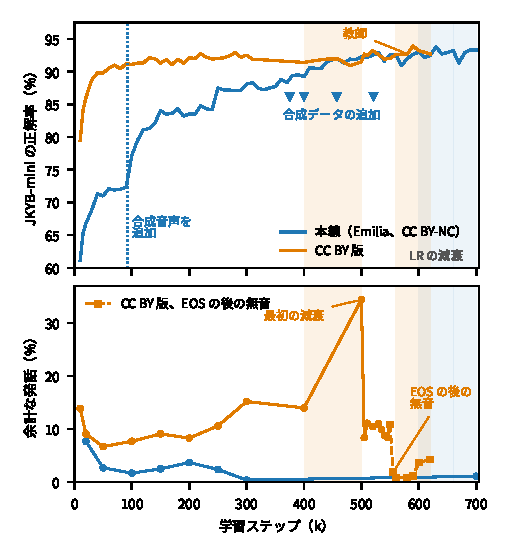
\includegraphics[width=\columnwidth]{fig_training_ja.pdf}
\caption{学習中の教師（CFG 2.0）。上: 読みの正答率は、ステップを重ねたときではなく、新しい合成データが
入ったときに上がる。下: 文の後に余計な発話がある文の割合。CC BY 版では、データの掃除でも減衰でも
消えず、EOS の後のフレームを教えると消えた。網掛け: 学習率の減衰。}
\label{fig:training}
\end{figure}

\textbf{ステップではなくデータ。}本線の教師は 3 回頭打ちになり（70--72\%、83.5--85\%、87.5--88\%）、
どれも新しい合成セットが入って初めて抜けた（図~\ref{fig:training}）。検証損失はこの改善を示さず、
JKYB-mini が 5\pt{} 上がった 93k と 100k のステップで同じ値だった。最後の cosine 減衰
（600k$\to$660k）で JKYB-mini が 0.6\pt、青空文庫が 4.6\pt{} 上がった（JSUT の CER は 2.86 から 2.40\%）。
最初から合成データを使った CC BY 版の教師は、35k ステップで 90\% に達した。

\subsection{発話の終わり方}\label{sec:end}
\textbf{短いチャンク。}172 個の短い文で、660k の本線の教師は 58 文の後に余計な発話を加え、22 文で
止まらなかった（CER 28\%）。S9 を時間で 1\% 混ぜた短文の段（40k ステップ、学習率を上げ直して減衰）で、
5k ステップのうちにどちらも直った（1 文と 1 文、CER 4.8\%）。

\textbf{EOS の後のフレーム。}CC BY 版の教師は、JKYB-mini の文の 7--15\% の後にフィラー（「うん」「えー」）
を加えていた。本線の 3--5 倍で、最初の減衰で 34\% に増えた。データでの対策は、どれも 7--11\% 付近で
止まった。YODAS3 のクリップの終わりの切り詰め、YODAS3 の ASR での再チェック、フィラーの除去、YODAS3
そのものの除去でさえそうだった（7.1\%、話者の類似度は 0.545 から 0.500 に低下）。EOS の後のフレームを
生成しないと、8.8\% が 3.3\% になった。フィラーの大半は、実行系が足す 5 フレームの中にあった。上流の
学習は最後の発話フレームより後で損失をマスクするので、このフレームは一度も学習されない。そこで、
すべての完結した目標の後にデジタル無音（ゼロを符号化した Mimi の潜在表現）を 6 フレーム足し、フローの
損失をかけた。EOS の目標は発話の終わりのままとする。10k ステップのうちに、余計な発話は 10.9\% から
0.9\%（本線は 1.1\%）、文の CER は 3.6--3.9\% から 1.9\%、短文の CER は 11.8\% から 5.2\% になり、EOS の
損失も速度も変わらなかった。続く減衰の後半では、今度は EOS の前にフィラーが戻った（620k で 4.3\%）ので、
教師には 580k のチェックポイントを使う。

\section{蒸留}\label{sec:distill}
\textbf{ガイダンス。}CFG なしでは、教師は 1.2\pt{} 読みが悪く、止まらない文が増え、3.9\,LU 小さかった。
スケールは 2.0 が最もよく読んだ（93.0\%、2.5 では 90.5\%）。実行系に CFG がないので、24 層の教師の複製に、
凍結した教師のガイダンス後の状態 $z_\varnothing+2(z_c-z_\varnothing)$ を学ばせる（トランスフォーマーの
出力の MSE、ヘッドは凍結、50k ステップ）。結果はガイダンス付きの教師より少しよく読み、
\texttt{japanese\_24l} として公開した。

\textbf{深さ。}6 層の生徒は上流の深さの蒸留に従う。教師の 0, 1, 2, 21, 22, 23 層から始め（上流は外側の層
が最良の初期値と報告している）、ガイダンス後の状態を学ぶ（本線は 42k + 120k ステップ、CC BY 版は
160k）。JKYB の全文で生徒は教師を\emph{上回る}。本線は 94.15 / 94.73\% に対して教師 92.97 /
93.68\%、CC BY 版は 93.93 / 93.96\% に対して 92.82 / 93.82\%（プロンプトは交代 / jvs001、元の
デコーダ）で、上流の英語の生徒でも同じことが起きている（WER 0.76\% と 0.82\%）。止まらない文は多い
（13,536 文中 43 文、教師は 6 文）。bfloat16 の 6 層モデルは、CPU 1 スレッドで実時間の 4.4 倍で動く
（24 層は 1.4 倍）。

\textbf{公開時の EOS の後のフレーム数。}クリップの終わりを音量で調べると、24 層の CC BY 版では、短い
終わりの音の半分が EOS の後にあった（クリップの 10.1\%、鳴ったまま切れるもの 2.5\%）。3 フレームに
すると 7.9\%、切れるもの 0.7\% になる（0 フレームでは 5.9\% だが 16\% が切れる）ので、設定を 3 とした。
6 層の音は EOS の前にあり（どの設定でも 9.4--9.8\%）、試聴でも気にならなかったので既定のままとした。

\section{デコーダの微調整}\label{sec:decoder}
\textbf{なぜ必要か。}JVS~\cite{jvs} の読み上げ全体を Mimi に通すと、かな CER は 3.16\% から 5.45\% に
上がる。増えるのは主に調音位置の変わる子音（キ$\to$チ、ガ$\to$ダ）である。子音の分類器は潜在表現から
94.1\% を当てるが、デコードした音声からは 92.0\% で、情報を失うのはデコーダである。そこでデコード側
（1,030 万パラメータ）だけを学習する。エンコーダ、潜在表現、言語モデル、声のプロンプトはそのままで、
実行系は新しいデコーダを同じ重みファイルから読む。

\textbf{本線。}損失は多重解像度のメル、MPD~\cite{hifigan} と MS-STFT~\cite{encodec} の識別器、
アップサンプリングのストライドの周波数（200\,Hz と 1.2\,kHz の倍数）に立つ音に対する、バッチで平均した
スペクトルの損失である。データは合成音声 182\,時間と高ビットレートの Emilia 60\,時間とした。指標は
すべて改善したが、試聴では 2 つのデコーダが、子音の金属的な音と、ピッチに同期した高域のために却下
された。4\,kHz より上で、録音には倍音がある所に雑音を出していた。最後の 10k ステップでこの帯域を元の
デコーダの出力に合わせると（\emph{keep4k}）、耳での問題が消え、改善は保たれた（表~\ref{tab:decoder}）。

\textbf{高域。}研究用のブランチで、4\,kHz より上をスタジオ録音~\cite{hificaptain,jvnv} に近づける
学習をした。指標のうち試聴の判定すべてと一致したのは、全ファイルに 40\,Hz のハイパスをかけた
UTMOSv2~\cite{utmosv2} だけだった（UTMOS22~\cite{utmos} は順位相関 $-0.86$、ViSQOL~\cite{visqol} は
却下されたデコーダを 1 位にした）が、それでも耳で聞こえた機械的な音は測れなかった。F0 ヘッドによる
倍音の励振は聴感が悪く、推論コードの追加も要る。デコーダを広げても変わらない。順位は学習データ
自体の予測 MOS で決まり、異なるレシピの run の平均~\cite{soups} が最良だったが、NC と継承条件付きの
データを使う。

\textbf{CC BY 版のデコーダ。}使えるのは元の Mimi、YODAS3、CC BY の声の合成音声だけである。YODAS3 の
クリップを、15\,kHz まで音があり DNSMOS の高い動画から 24\,kHz で切り出し直し（9 万クリップ、
234\,時間）。クリップの選択は、UTMOSv2 の順位は効き、
倍音の強さは効かなかった。土台は元の Mimi から YODAS3 164\,時間と合成音声 116\,時間で 70k ステップ
（識別器も一から）学習し、その上で帯域の欠けやクリッピングのない UTMOSv2 の上位のクリップ（7--14\,時間）で高域を学ぶ 10k ステップの
run を 4 本回して平均した。試聴で合成音声と分かった YODAS3 の動画 2 本は除いた。結果は再構成で NC の最良
のデコーダと並び、TTS では少し上回る（元の Mimi より UTMOSv2 +0.35--0.42、話者の類似度
0.55$\to$0.65）。試聴では CC BY 版のデコーダとの区別はつかなかった。

\begin{table}[t]
\centering\footnotesize\setlength{\tabcolsep}{3pt}
\caption{JVS の再構成（10 話者 $\times$ 100 文）でのデコーダ。UTMOSv2 は keep4k との差。}
\label{tab:decoder}
\begin{tabular}{@{}lrrrl@{}}
\toprule
デコーダ & CER & 類似度 & UTMOSv2 & データ\\
\midrule
録音 & 3.34 & -- & +0.400 &\\
元の Mimi & 5.44 & 0.698 & $-0.036$ &\\
keep4k（本線の公開版） & 4.70 & 0.779 & 0 & NC\\
最良の平均（研究用） & 4.74 & 0.784 & +0.397 & NC、SA\\
CC BY（\texttt{M2CH2\_soup4}） & 4.69 & 0.805 & +0.383 & CC BY\\
\bottomrule
\end{tabular}
\end{table}

\section{公開したモデル}\label{sec:results}
公開したモデルを表~\ref{tab:results} に示す。生成した音声を kana-whisper で書き起こして評価する。
JKYB-Parakeet~\cite{jkyb,jkybp}（対象語に印を付けた 13,536 文。プロンプトは JVS の 4 話者の交代、
または jvs001）、その 1,500 文の部分集合 JKYB-mini、合成に使っていない作品の青空文庫のルビ 1,000 語、
JSUT~\cite{jsut} の 1,000 文、JVS の 10 話者のゼロショットのクローン（かな CER と、その話者が同じ文を
読んだ録音との ECAPA の類似度）、短い文 172 個である。JVS と JSUT は学習に使わない。公開したファイルを
公式パッケージで CPU で読み込んでも、揺れの範囲で同じになる（本線の \texttt{japanese}: JKYB-mini
95.3\%、JSUT 2.15\%、JVS 1.70\% / 0.575）。

\begin{table}[t]
\centering\scriptsize\setlength{\tabcolsep}{1.3pt}
\caption{公開したモデル（GPU での評価。L: 層、教師は CFG 2.0）。JKYB: 全文、プロンプトは交代 /
jvs001。CER は \%。短文: 止まらない / 余計な発話（172 文中）。\tbd{赤}: 暫定。}
\label{tab:results}
\begin{tabular}{@{}lrrrrrr@{}}
\toprule
モデル & JKYB & mini & 青空 & JSUT & JVS / 類似度 & 短文\\
\midrule
\multicolumn{7}{@{}l}{\emph{本線（CC BY-NC）、デコーダ keep4k}}\\
6L & 94.75 / 94.84 & 95.1 & 71.3 & 2.28 & 2.32 / .577 & 0 / 1\\
24L & 94.32 / 94.49 & 94.5 & 71.2 & 2.28 & 2.13 / .586 & 0 / 1\\
\multicolumn{7}{@{}l}{\emph{CC BY 版、CC BY のデコーダ}}\\
6L & \tbd{94.77 / TBD} & 94.9 & 70.7 & 2.14 & 2.18 / .651 & \tbd{0 / TBD}\\
24L & \tbd{TBD} & \tbd{TBD} & \tbd{TBD} & \tbd{TBD} & \tbd{TBD} & \tbd{TBD}\\
\multicolumn{7}{@{}l}{\emph{元の Mimi のデコーダ}}\\
本線 6L & 94.15 / 94.73 & 93.8 & 70.0 & 2.39 & 2.58 / .536 & 0 / 1\\
CC BY 6L & 93.93 / 93.96 & 94.3 & 69.0 & 2.40 & 2.47 / .560 & 0 / 1\\
CC BY 24L & 93.34 / 94.08 & 93.5 & 68.5 & 2.48 & 2.67 / .547 & 0 / 0\\
本線の教師 & 92.97 / 93.68 & 93.3 & 69.4 & 2.66 & 3.05 / -- & 1 / 2\\
CC BY の教師 & 92.82 / 93.82 & 92.7 & 67.9 & 2.58 & 2.45 / .546 & 0 / --\\
\bottomrule
\end{tabular}
\end{table}

専用のデコーダで、半分のデータの CC BY 版も本線に並ぶ。どちらの 6 層も JKYB の約 5\% を読み誤り、多くは
まれな読みと熟字訓である。

\section{議論}
\textbf{効いたこと。}第一に\emph{網羅性}。モデルは十分な回数聞いた読みだけを覚える。読みの正しい TTS
モデルの合成音声を ASR で確かめたものが最も安くそれを補う。ただし確認が難しい読みを捨ててはいけない。
第二に\emph{実行系がすることを学習させる}。EOS の後のフレーム、短いチャンク、CFG がないことは、それぞれ
教えるか蒸留する必要があった。第三に\emph{デコーダは指標だけでは決められない}。却下したデコーダは
どれも、すべての指標を改善していた。

\textbf{限界。}スコアは ASR に基づき、乱数は 1 通りで、JKYB-mini は評価ごとに約 $\pm$0.5--1\pt{} 動く。
合成データの割合を制御した比較はしていない。合成音声には Irodori の読みと話し方が乗る。生徒は教師より
少し止まらない文が多く、CC BY 版のクリップの 8--10\% は短く静かな音で終わる。

\section{おわりに}
日本語の Pocket TTS は、実行系を変えずに作れる。改善の大半はデータから来た。ASR で再チェックした Web の
音声、揃えた音量、まれな読みを補う合成音声である。実行系が EOS の後に生成するフレームを教えると文末の
フィラーが消え、蒸留で教師よりよく読む 6 層のモデルができ、CC BY の音声で微調整したデコーダで、CC BY
版は Emilia を使った版に並んだ。

\section*{謝辞}
Pocket TTS と学習コードを公開した Kyutai と、Emilia、YODAS3、Irodori-TTS、JKYB と Parakeet 版、
kana-whisper、JSUT、JVS、Hi-Fi-CAPTAIN、JVNV、UTMOSv2、青空文庫、Wikipedia、Tatoeba、EDRDG の
辞書の作成者に感謝する。

\begin{thebibliography}{99}\footnotesize
\setlength{\itemsep}{0pt}
\bibitem{pocket} M.~Orsini, S.~Rouard, G.~De~Marmiesse, V.~Volhejn, N.~Zeghidour, A.~Défossez.
Pocket TTS. \url{https://github.com/kyutai-labs/pocket-tts}, 2026.
\bibitem{calm} S.~Rouard, M.~Orsini, A.~Roebel, N.~Zeghidour, A.~Défossez. Continuous audio
language models. \emph{ICLR}, 2026.
\bibitem{mar} T.~Li, Y.~Tian, H.~Li, M.~Deng, K.~He. Autoregressive image generation without vector
quantization. \emph{NeurIPS}, 2024.
\bibitem{lsd} N.~M.~Boffi, M.~S.~Albergo, E.~Vanden-Eijnden. How to build a consistency model:
Learning flow maps via self-distillation. \emph{NeurIPS}, 2025.
\bibitem{cfg} J.~Ho, T.~Salimans. Classifier-free diffusion guidance. arXiv:2207.12598, 2022.
\bibitem{moshi} A.~Défossez et al. Moshi: a speech-text foundation model for real-time dialogue.
arXiv:2410.00037, 2024.
\bibitem{emilia} H.~He et al. Emilia: An extensive, multilingual, and diverse speech dataset for
large-scale speech generation. \emph{SLT}, 2024.
\bibitem{emilialarge} H.~He et al. Emilia: A large-scale, extensive, multilingual, and diverse
dataset for speech generation. arXiv:2501.15907, 2025.
\bibitem{ecapa} B.~Desplanques, J.~Thienpondt, K.~Demuynck. ECAPA-TDNN: Emphasized channel
attention, propagation and aggregation in TDNN based speaker verification. \emph{Interspeech}, 2020.
\bibitem{dnsmos} C.~K.~A.~Reddy, V.~Gopal, R.~Cutler. DNSMOS P.835: A non-intrusive perceptual
objective speech quality metric to evaluate noise suppressors. \emph{ICASSP}, 2022.
\bibitem{yodas} X.~Li et al. YODAS: YouTube-oriented dataset for audio and speech. \emph{ASRU}, 2023.
\bibitem{yodas3} W.~Chen, S.~Takamichi, S.~Shiota, S.~Fukayama, S.~Cornell, S.~Watanabe. YODAS v3:
Over 1 million hours of high-bandwidth, stereophonic, multilingual speech. \emph{Interspeech}, 2026.
\bibitem{silero} Silero Team. Silero VAD. \url{https://github.com/snakers4/silero-vad}.
\bibitem{whisper} A.~Radford et al. Robust speech recognition via large-scale weak supervision.
\emph{ICML}, 2023.
\bibitem{kanawhisper} SB Intuitions. \texttt{sbintuitions/kana-whisper}. Hugging Face.
\bibitem{yomi} Claude, 森 琢磨. フローマッチング TTS に漢字の読みを教える. テクニカルレポート, 2026.
\bibitem{jmdict} J.~Breen. JMdict: a Japanese-multilingual dictionary. \emph{COLING Workshop on
Multilingual Linguistic Resources}, 2004.
\bibitem{sentencepiece} T.~Kudo, J.~Richardson. SentencePiece: A simple and language independent
subword tokenizer and detokenizer for neural text processing. \emph{EMNLP (demo)}, 2018.
\bibitem{hifigan} J.~Kong, J.~Kim, J.~Bae. HiFi-GAN: Generative adversarial networks for efficient
and high fidelity speech synthesis. \emph{NeurIPS}, 2020.
\bibitem{encodec} A.~Défossez, J.~Copet, G.~Synnaeve, Y.~Adi. High fidelity neural audio
compression. \emph{TMLR}, 2023.
\bibitem{hificaptain} NICT. Hi-Fi-CAPTAIN corpus.
\url{https://ast-astrec.nict.go.jp/en/release/hi-fi-captain/}.
\bibitem{jvnv} D.~Xin et al. JVNV: A corpus of Japanese emotional speech with verbal content and
nonverbal expressions. \emph{IEEE Access}, 2024.
\bibitem{utmosv2} K.~Baba, W.~Nakata, Y.~Saito, H.~Saruwatari. The T05 system for the VoiceMOS
Challenge 2024. \emph{SLT}, 2024.
\bibitem{utmos} T.~Saeki et al. UTMOS: UTokyo-SaruLab system for VoiceMOS Challenge 2022.
\emph{Interspeech}, 2022.
\bibitem{visqol} M.~Chinen et al. ViSQOL v3: An open source production ready objective speech and
audio metric. \emph{QoMEX}, 2020.
\bibitem{soups} M.~Wortsman et al. Model soups: averaging weights of multiple fine-tuned models
improves accuracy without increasing inference time. \emph{ICML}, 2022.
\bibitem{jvs} S.~Takamichi et al. JVS corpus: free Japanese multi-speaker voice corpus.
arXiv:1908.06248, 2019.
\bibitem{jkyb} SB Intuitions. Joyo Kanji Yomi Benchmark.
\url{https://github.com/sbintuitions/Joyo-Kanji-Yomi-Benchmark}.
\bibitem{jkybp} Parakeet Inc. Joyo Kanji Yomi Benchmark, Parakeet Edition.
\url{https://github.com/Parakeet-Inc/Joyo-Kanji-Yomi-Benchmark-Parakeet-Edition}.
\bibitem{jsut} R.~Sonobe, S.~Takamichi, H.~Saruwatari. JSUT corpus: free large-scale Japanese
speech corpus for end-to-end speech synthesis. arXiv:1711.00354, 2017.
\end{thebibliography}
\end{document}
